%%%%%%%%%%%%%%%%%%%%%%%%%%%%%%%%%%%%%%%%%
% Beamer Presentation
% LaTeX Template
% Version 1.0 (10/11/12)
%
% This template has been downloaded from:
% http://www.LaTeXTemplates.com
%
% License:
% CC BY-NC-SA 3.0 (http://creativecommons.org/licenses/by-nc-sa/3.0/)
%
%%%%%%%%%%%%%%%%%%%%%%%%%%%%%%%%%%%%%%%%%

%----------------------------------------------------------------------------------------
%	PACKAGES AND THEMES
%----------------------------------------------------------------------------------------

\documentclass{beamer}

\mode<presentation> {

% The Beamer class comes with a number of default slide themes
% which change the colors and layouts of slides. Below this is a list
% of all the themes, uncomment each in turn to see what they look like.

%\usetheme{default}
%\usetheme{AnnArbor}
%\usetheme{Antibes}
%\usetheme{Bergen}
%\usetheme{Berkeley}
%\usetheme{Berlin}
%\usetheme{Boadilla}
%\usetheme{CambridgeUS}
%\usetheme{Copenhagen}
%\usetheme{Darmstadt}
%\usetheme{Dresden}
%\usetheme{Frankfurt}
%\usetheme{Goettingen}
%\usetheme{Hannover}
%\usetheme{Ilmenau}
%\usetheme{JuanLesPins}
%\usetheme{Luebeck}
%
\usetheme{Madrid}
%\usetheme{Malmoe}
%\usetheme{Marburg}
%\usetheme{Montpellier}
%\usetheme{PaloAlto}
%\usetheme{Pittsburgh}
%\usetheme{Rochester}
%\usetheme{Singapore}
%\usetheme{Szeged}
%\usetheme{Warsaw}

% As well as themes, the Beamer class has a number of color themes
% for any slide theme. Uncomment each of these in turn to see how it
% changes the colors of your current slide theme.

%\usecolortheme{albatross}
%\usecolortheme{beaver}
%\usecolortheme{beetle}
%\usecolortheme{crane}
%\usecolortheme{dolphin}
%\usecolortheme{dove}
%\usecolortheme{fly}
%\usecolortheme{lily}
%\usecolortheme{orchid}
%\usecolortheme{rose}
%
\usecolortheme{seagull}
%\usecolortheme{seahorse}
%\usecolortheme{whale}
%\usecolortheme{wolverine}

%\setbeamertemplate{footline} % To remove the footer line in all slides uncomment this line
%\setbeamertemplate{footline}[page number] % To replace the footer line in all slides with a simple slide count uncomment this line

%\setbeamertemplate{navigation symbols}{} % To remove the navigation symbols from the bottom of all slides uncomment this line
}

\usepackage{graphicx} % Allows including images
\usepackage{booktabs} % Allows the use of \toprule, \midrule and \bottomrule in tables
\usepackage{tikz}





\usepackage[ final ]{pdfpages}
%----------------------------------------------------------------------------------------
%	TITLE PAGE
%----------------------------------------------------------------------------------------

\title[SWOP iteratie 1]{SWOP iteratie 1} % The short title appears at the bottom of every slide, the full title is only on the title page

\author{Groep 8} % Your name
\institute[KULeuven] % Your institution as it will appear on the bottom of every slide, may be shorthand to save space
{\\ % Your institution for the title page
\medskip
\textit{} % Your email address
}
\date{} % Date, can be changed to a custom date
\usepackage{graphicx}
\usepackage{caption}
\usepackage{subcaption}
\begin{document}

\begin{frame}
\titlepage % Print the title page as the first slide
\end{frame}


%----------------------------------------------------------------------------------------
%	PRESENTATION SLIDES
%----------------------------------------------------------------------------------------


\begin{frame}
\frametitle {General overview}

\begin{figure}[!htb]
    \centering
    \begin{tikzpicture}
        \node[anchor=south west,inner sep=0] (image) at (0,0) {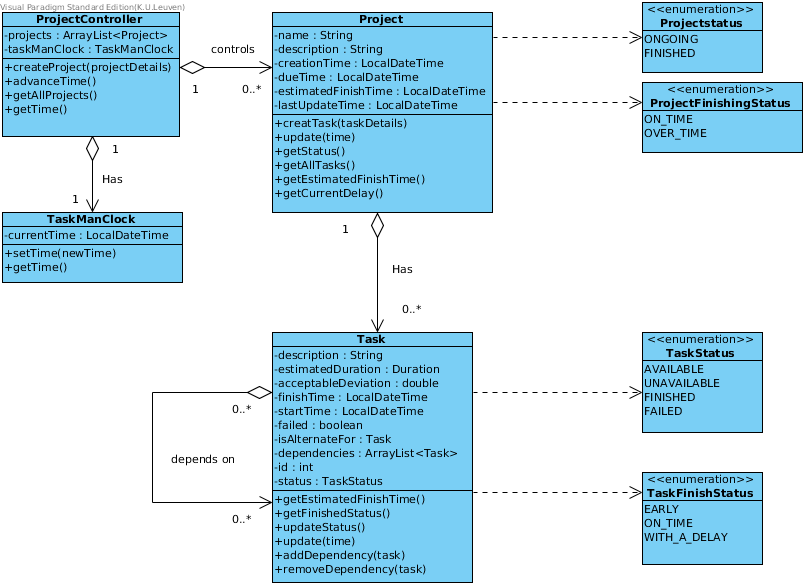
\includegraphics[width=\textwidth]{/home/travolter/SWOP-groep-8/Presentatie_iteratie1/figures/Class_Diagram.png}};
        \begin{scope}[x={(image.south east)},y={(image.north west)}]
            \draw[help lines,xstep=.1,ystep=.1] (0,0) grid (1,1);
            \foreach \x in {0,1,...,9} { \node [anchor=north] at (\x/10,0) {0.\x}; }
            \foreach \y in {0,1,...,9} { \node [anchor=east] at (0,\y/10) {0.\y}; }
            \node[anchor=south west,inner sep=0] (image) at (0.5,0.7) {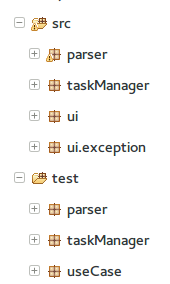
\includegraphics[width=0.1\textwidth]{/home/travolter/SWOP-groep-8/Presentatie_iteratie1/figures/Package_overview.png}};
        \end{scope}
    \end{tikzpicture}
    \caption{Find that penguin!}
\end{figure}
\end{document}

\end{frame}


\begin{frame}
\frametitle {\texttt{ProjectController} - GRASP}


\end{frame}

\begin{frame}
\frametitle {\texttt{Project} en \texttt{Task}- GRASP}


\end{frame}


\begin{frame}
\frametitle {Tijd}


\end{frame}

\begin{frame}
\frametitle {Extensions}


\end{frame}

\begin{frame}
\frametitle {Testing}


\end{frame}
\end{document} 
